\documentclass[11pt,a4paper]{article}
\usepackage[utf8]{inputenc}
\usepackage[T1]{fontenc}
\usepackage[french]{babel}
\usepackage{lmodern}
\usepackage[margin=1.7cm,headheight=14pt]{geometry}
\usepackage{graphicx}
\graphicspath{{outputs/}{./}}
\usepackage{booktabs,tabularx}
\usepackage{xcolor}
\usepackage{hyperref}
\usepackage{fancyhdr}
\usepackage{titlesec}
\usepackage{float}
\definecolor{navy}{HTML}{18324B}
\definecolor{blue}{HTML}{2F6B8A}
\definecolor{pale}{HTML}{EAF1F5}
\hypersetup{colorlinks=true,linkcolor=blue,urlcolor=blue}
\titleformat{\section}{\large\bfseries\color{navy}}{\thesection}{0.6em}{}
\pagestyle{fancy}\fancyhf{}
\fancyhead[L]{\small\color{navy}Pricing paramétrique séisme}
\fancyhead[R]{\small Étude de modélisation}
\fancyfoot[C]{\thepage}
\setlength{\parskip}{5pt}
\setlength{\parindent}{0pt}

\title{\vspace{-1.1cm}\Huge\bfseries\color{navy}Pricing d'une couverture\\[3pt]
\Large paramétrique séisme\\[7pt]
\normalsize Simulation, tarification et basis risk}
\author{Projet de modélisation actuarielle en Python}
\date{6 novembre 2026}

\begin{document}
\maketitle
\vspace{-0.5cm}
\colorbox{pale}{\parbox{\dimexpr\textwidth-2\fboxsep}{\textbf{En bref.} Ce prototype simule l'aléa sismique, transforme le PGA en indemnités contractuelles, puis mesure le prix, le risque extrême et le décalage possible entre indemnité et perte. Les paramètres sont stylisés et ne sont pas calibrés sur une région réelle.}}

\section{Comment fonctionne le modèle ?}
\begin{center}
\fcolorbox{blue}{white}{\parbox{0.88\textwidth}{\centering
Séismes simulés (fréquence, magnitude, distance)\\[3pt]
\Large$\downarrow$\\[-2pt]
PGA à la station de référence\\[-1pt]
\Large$\downarrow$\\[-2pt]
Indemnité en paliers, agrégée par année\\[-1pt]
\Large$\downarrow$\\[-2pt]
Prime, VaR/TVaR, basis risk et sensibilités}}
\end{center}
Le PGA est l'accélération maximale du sol. La couverture est paramétrique : elle paie selon cet indice, sans mesurer directement les dommages assurés. La limite annuelle est de 10 M\$; les paliers paient 25\%, 50\% et 100\% aux seuils 0,08 g, 0,15 g et 0,25 g.

\begin{figure}[H]\centering
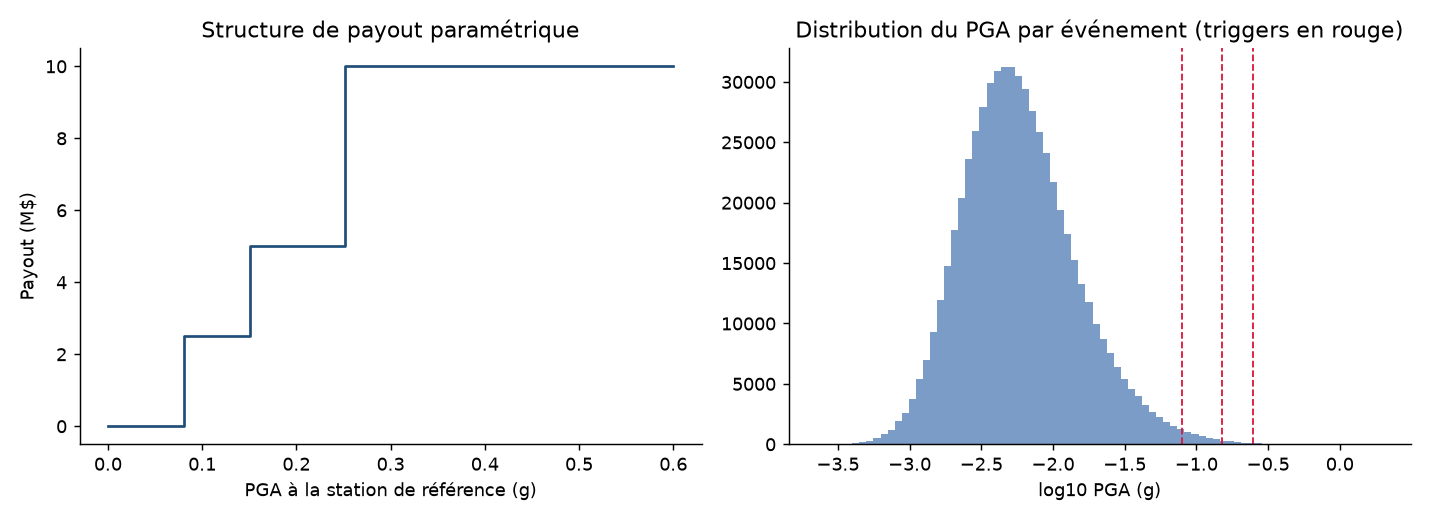
\includegraphics[width=0.91\textwidth,height=5.2cm,keepaspectratio]{fig1_payout_pga.png}
\caption{Structure de paiement et distribution de PGA simulée.}\end{figure}

\section{Résultats principaux}
L'étude couvre 200\,000 années simulées. La probabilité annuelle de paiement est de 2,518\%. L'indemnité annuelle moyenne (AAL) atteint 88\,475\$; la prime par principe de l'écart-type ajoute 35\% de l'écart-type des paiements :
\[
\text{Prime}=88\,475 + 0{,}35\times639\,032 = 312\,136\ \$.
\]
Le rate on line, soit la prime divisée par la limite de 10 M\$, est de 3,12\%.

\begin{center}\renewcommand{\arraystretch}{1.22}
\begin{tabularx}{0.9\textwidth}{Xr}
\toprule\textbf{Mesure} & \textbf{Résultat}\\\midrule
VaR 99\% & 2,50 M\$\\
TVaR 99\% & 5,05 M\$\\
Prime coût du capital (variante) & 584,75 k\$\\
Prime P5--P95 après réestimation & 258,5--378,9 k\$\\
\bottomrule
\end{tabularx}\end{center}
La TVaR est la moyenne des 1\% d'années les plus coûteuses. Le calcul sélectionne exactement cette fraction, y compris quand plusieurs années ont le même montant de paiement.

\begin{figure}[H]\centering
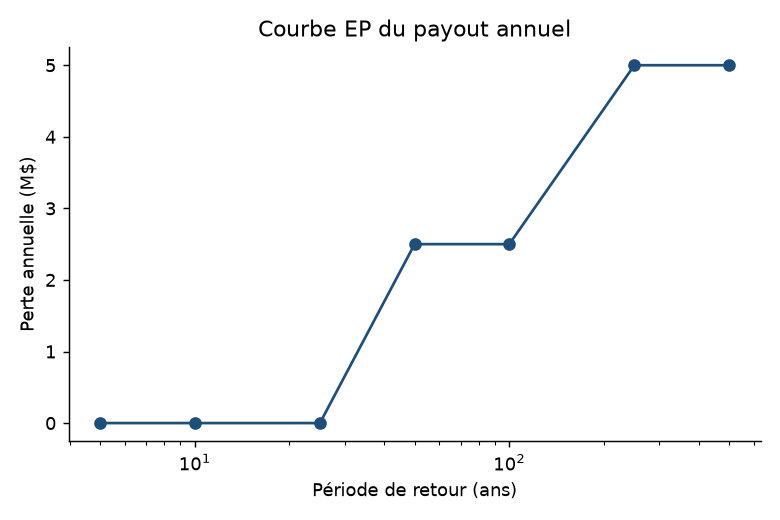
\includegraphics[width=0.70\textwidth,height=5.0cm,keepaspectratio]{fig2_ep_curve.png}
\caption{Courbe de dépassement des paiements annuels (EP).}\end{figure}

\section{Incertitude et qualité de l'indice}
Pour illustrer l'incertitude paramétrique, 200 catalogues fictifs de 60 ans sont créés; la fréquence et la b-value sont réestimées avant le repricing. Le coefficient de variation des primes est de 11,6\%. Cet exercice mesure une incertitude sous le modèle retenu, pas une incertitude empirique sur un portefeuille réel.

\begin{figure}[H]\centering
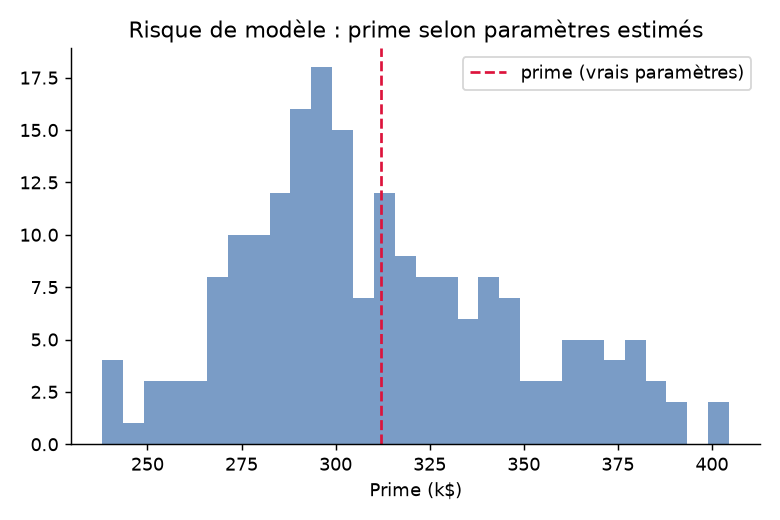
\includegraphics[width=0.72\textwidth,height=4.4cm,keepaspectratio]{fig3_param_uncertainty.png}
\caption{Distribution de prime issue des catalogues pseudo-observés.}\end{figure}

Le modèle compare ensuite la perte simulée au paiement de l'indice. La corrélation est de 0,682. Dans 1,395\% des années, le contrat paie alors que la perte est sous le seuil matériel retenu; dans 0,238\% des années, une perte matérielle survient sans paiement. Ce décalage est le \textit{basis risk}. Le seuil matériel (5\% de la limite) est une convention du modèle.

\section{Choix du trigger et sensibilités}
Pour les couvertures binaires testées, un seuil plus élevé réduit la fréquence de paiement et la prime, mais augmente le risque de perte matérielle sans indemnité. Sur la grille calculée, les fréquences des deux types d'erreur changent d'ordre entre 0,12 g et 0,16 g; le point d'égalité n'est pas déterminé plus précisément.

\begin{figure}[H]\centering
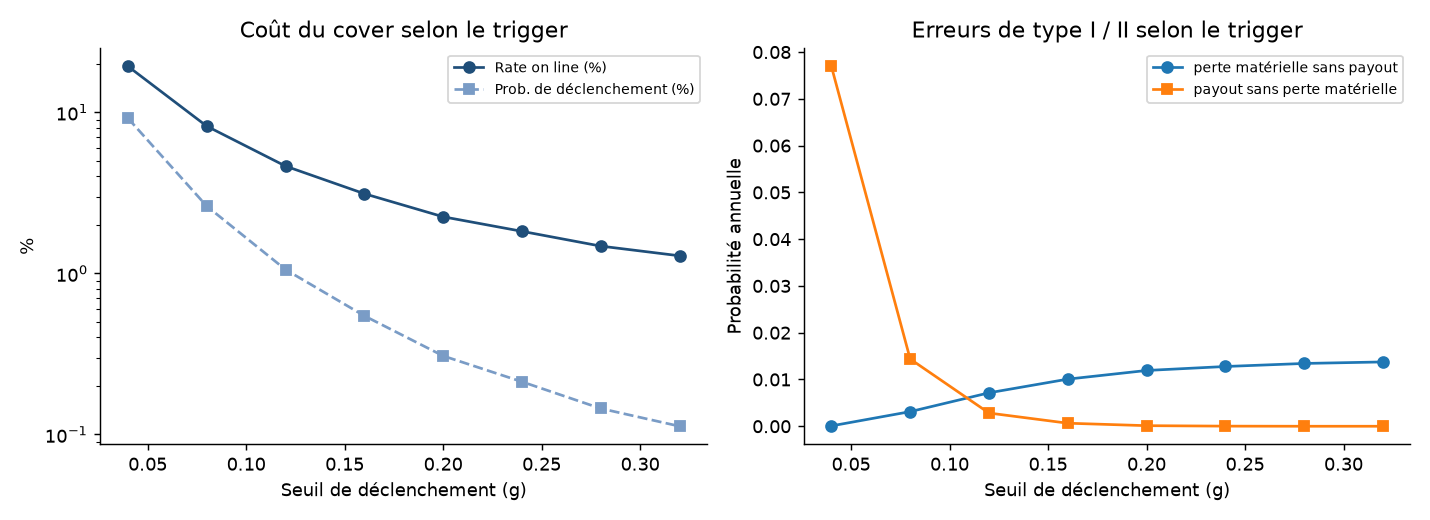
\includegraphics[width=0.90\textwidth,height=5.0cm,keepaspectratio]{fig4_trigger_frontier.png}
\caption{Coût du contrat et erreurs selon le seuil de déclenchement.}\end{figure}

Les scénarios de sensibilité varient une hypothèse à la fois. Le coefficient d'atténuation $c_2$ de la GMPE a l'effet le plus marqué : de $-22,7\%$ à $+39,2\%$ sur la prime. La variation de $\sigma$ de la GMPE donne $-16,2\%$ à $+19,2\%$.

\begin{figure}[H]\centering
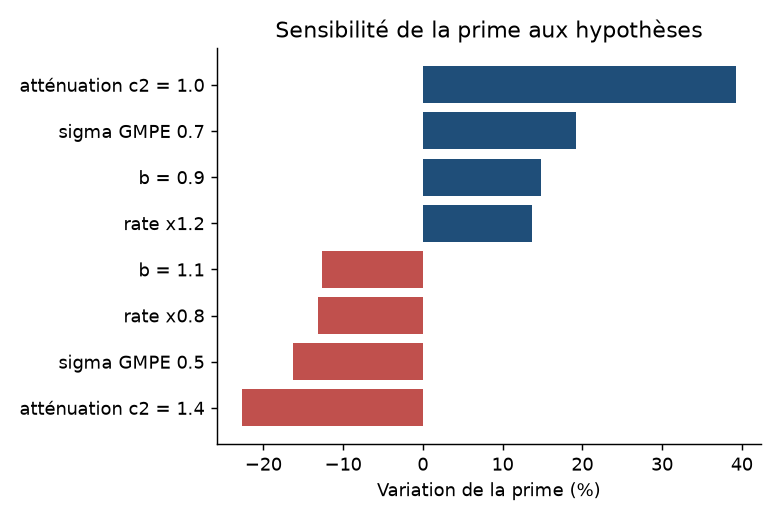
\includegraphics[width=0.72\textwidth,height=4.4cm,keepaspectratio]{fig5_sensitivity.png}
\caption{Variation de la prime dans les scénarios étudiés.}\end{figure}

\section{Conclusion et limites}
Le projet démontre une chaîne Python de modélisation et de tarification paramétrique, avec analyse de l'incertitude, du basis risk, des seuils et des sensibilités. Le résultat le plus important est la dépendance du prix aux hypothèses de la GMPE.

Le catalogue d'événements, la relation PGA et la vulnérabilité sont stylisés; aucune calibration régionale ni validation sur pertes réelles n'a été menée. Avant un usage réel, il faudrait intégrer un catalogue historique et une GMPE publiée adaptés à une région, puis calibrer la vulnérabilité sur le portefeuille.

\vfill\small\textit{Résultats reproductibles avec la graine fixée dans le projet. Ce document présente un exercice de modélisation; il ne constitue pas une cotation commerciale.}
\end{document}
